\section{Data}\label{data}
\subsection{Data Source \& Collection}
Our data is collected from four different sources:

\emph{UFO Sighting Data}, the majority of our data set, is from National UFO Report Center~\cite{nuforc}. It is composed by 96000 UFO sighting reports and each report contains information of event date (year, month, day, hour), city, state, shape, duration, sighting description and posted date. Since this website doesn't provide an API to access the data, we implement a web crawler to collect data from its web pages. 

\emph{Geo Information Data} is collected from Google Map~\cite{googlemap} which provides well-developed APIs for developers to obtain comprehensive information. We first filter out cities where UFO events happened, and then obtain longitude and latitude information of these cities. In total, about 19000 records of geo information have been collected. 

\emph{Weather Data} is collected from DarkSky website~\cite{darksky}. We collect weather conditions (icon, temperature, apparent temperature, dew point, humidity, wind speed, wind bearing, visibility and pressure) when UFO events happened. Weather data has the same size with UFO sighting data.

\emph{U.S. Area/population Data} is from U.S. Census Bureau~\cite{census}. The data is downloaded manually and is stored in separate CSV files sorted by year.

\subsection{Data ETL}
A snapshot of raw UFO report data is as following:

\begin{figure}[H]
    \centering
    
\includegraphics[width=14cm]{figure/raw_event.jpg}
    \caption{raw UFO sighting data}
    \label{raw_event}
\end{figure}

We separate each fields, unify units of measurement (i.e. use seconds to measure any event duration), clean the summary, and remove records that contain invalid data elements. Also, in order to make further data processing easier, we complete the following steps for each summary field:

\begin{itemize}
    \item lowercase all characters
    \item strip punctuation
    \item remove all items in brackets
    \item apply Porter Stemming algorithm
\end{itemize}

And what's worth noting is that we use NUFORC's comments on each record's summary field to label report as true (1) or fake (0). 

In order to distinguish each data record in database, we assign an event\_id to each report data along with the weather data correlated to the sighting report. Each city is also assigned a location\_id. However, considering the growing data size and the way we use location information, city's latitude and longitude data are finally integrated into each report as two additional columns. Also, due to the size of reports and weather data, we store them in different data tables, although they share the same index event\_id. As for population and area data, since they are independent from UFO sightings, we create two other tables that do not have ids as indexes. Figure \ref{schema} shows the data schema of our database. 

\begin{figure}[H]
    \centering
    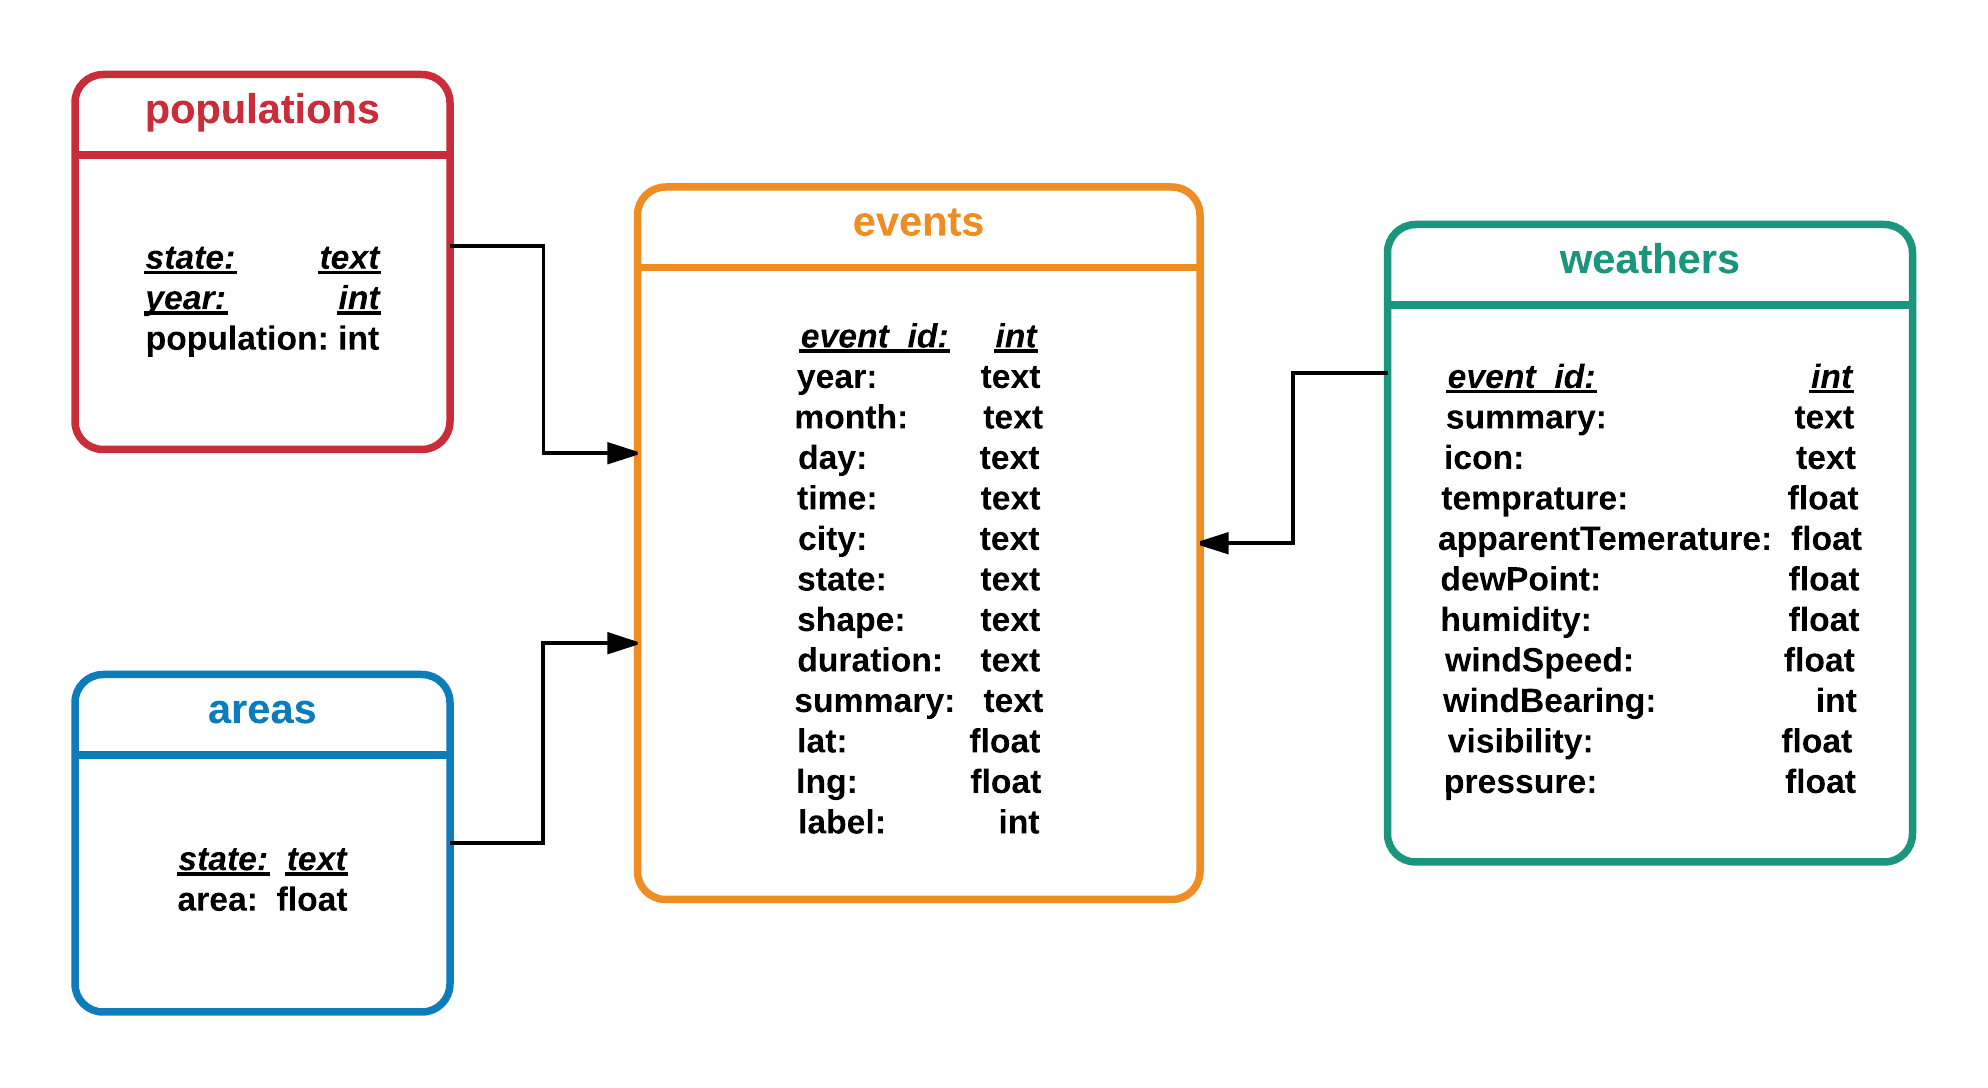
\includegraphics[width=14cm]{figure/schema.png}
    \caption{data schema of my\_ufo.db}
    \label{schema}
\end{figure}








